\documentclass{beamer}
%%%%%% UNOFFICIAL ICL BEAMER TEMPLATE V.0.1 %%%%%%

\usepackage[english]{babel}
\usepackage{amsmath,amssymb}
\usepackage{tikz}
\usetikzlibrary{arrows.meta,positioning,fit,backgrounds,calc}

%%%%%% THE FOLLOWING FILE CONTAINS THE STYLE DEFINITIONS %%%%%%
%%%%%% STYLE DEFINITIONS — inlined from the source deck's header.tex, so this
%%%%%% file is the whole deck (the build offers slides.tex as a download).
\usepackage[utf8]{inputenc}

\definecolor{gris}{rgb}{0.92,0.92,0.92}
\definecolor{blau-upc}{rgb}{.192,.365,.506}

\setbeamercolor{titlelike}{fg=blau-upc}
% \setbeamercolor{barra}{bg=white,fg=white}
\setbeamercolor{capcalera}{bg=blau-upc,fg=white}
\setbeamercolor{section in toc}{fg=blau-upc}
\setbeamertemplate{sections/subsections in toc}[circle]
\setbeamertemplate{itemize items}[circle]
\setbeamercolor{item}{fg=blau-upc}
\setbeamertemplate{blocks}[rounded][shadow=true]
\setbeamercolor*{block body}{bg=gris}
\setbeamerfont{block body}{size=\footnotesize}
\setbeamercolor*{block title}{parent=structure,bg=blau-upc,fg=white}

\setbeamersize{text margin left=12mm,text margin right=12mm}
\setbeamertemplate{navigation symbols}{}

\defbeamertemplate*{headline}{infolines theme}
{
	\begin{beamercolorbox}[wd=\paperwidth,ht=9.5mm,right]{white}%
		% (the ICL template's logo sat here; the empty box keeps the headline's height)
		\vskip0.2ex
	\end{beamercolorbox}
% 	\begin{beamercolorbox}[wd=\paperwidth,ht=0.5mm,left]{barra}%
% 		\hspace*{1mm}
% 	\end{beamercolorbox}
}

\setbeamertemplate{footline}
{
	\hbox{
	\begin{beamercolorbox}[wd=0.1\paperwidth,ht=10mm,left]{}
% 		\hspace*{1ex}\includegraphics[height=8mm]{./logotips/imperiallogo.pdf}\vskip 2ex
	\end{beamercolorbox}
	\begin{beamercolorbox}[wd=0.8\paperwidth,ht=3ex,center]{}
		\hspace*{4ex}\insertsection\vskip 4ex
	\end{beamercolorbox}
	\begin{beamercolorbox}[wd=0.1\paperwidth,ht=3ex,right]{}
		\insertpagenumber\hspace*{6ex}\vskip 4ex
	\end{beamercolorbox}
	}
}

\setbeamertemplate{title page}
{
	\vbox{}
	\vfill
	\begin{centering}
		{\usebeamerfont{title}\usebeamercolor[fg]{title}\inserttitle}
		\vskip0.2em
		{\usebeamerfont{subtitle}\usebeamercolor[fg]{subtitle}\insertsubtitle}
		\vskip2em\par
		\small\insertauthor\par
		\vskip0.7em\par
		\tiny\insertdate\vskip1em\par
	\end{centering}
% 	\vfill
}

% (the ICL template's background picture sat here)
%%%%%%
%%%%%%

%%%%%% TITLE, AUTHOR, DATE DEFINITIONS %%%%%%
\title{Decision Theory}
\author{Daniel C}
\date{}
%%%%%%

\begin{document}

\frame{\titlepage}

\frame{\frametitle{Roadmap}
	\begin{block}{From classical choice to embedded counterfactuals}
		{\tiny
		\begin{itemize}
			\item \textbf{Why decision theory matters for AI safety} (modelling, specification, reflective stability, multi-agent conflict)
			\item \textbf{Why it is hard:} optimisation is solved for \emph{dualistic} agents but not for \emph{embedded} ones, where the agent must \emph{construct} counterfactuals
			\item \textbf{The candidates:} causal (CDT), evidential (EDT), functional/logical (FDT), updateless (UDT 1.0, UDT 1.1) -- each is a different recipe for the counterfactual
			\item \textbf{A unifying lens:} CDT vs EDT as two readings of an action in sequential (AIXI-style) prediction -- an \emph{intervention} (chronological semimeasure) vs \emph{evidence} (joint prediction)
			\item \textbf{The hard core:} problems with UDT, the 5-and-10 problem, logical counterfactuals and L\"ob's theorem
			\item \textbf{A unifying goal:} formalise decision problems as programs and ask which decision theory is \emph{optimal} across all ``fair'' problems
		\end{itemize}
		}
	\end{block}
}

%==================================================================
\section{Why decision theory?}
%==================================================================

\frame{\frametitle{Why study decision theory? (for AI safety)}
	\begin{block}{Four reasons}
		{\tiny
		\begin{itemize}
			\item \textbf{Architecture-independent modelling.} We want to reason about how a superintelligent agent will \emph{behave} without knowing the details of how it is built. Decision theory is a minimal model of ``what is rational choice'', capturing behaviour any sufficiently capable agent tends to converge on.
			\item \textbf{Implementation / the specification--optimisation split.} Alignment decomposes into (1) \emph{specify} a goal we want, and (2) \emph{optimise} it correctly. Decision theory is part (2). A perfect specification is \textbf{not sufficient} for safety: if the agent constructs the wrong counterfactuals, it can ``optimise'' the goal in a way we never intended.
			\item \textbf{Reflective stability.} Safety properties must remain invariant under self-modification (cf.\ Agent Foundations deck). Decision theory is the simplest setting to ask: \emph{would an agent running decision theory A want to self-modify into, or build a successor with, decision theory B?} A decision theory that wants to overwrite itself is a warning sign.
			\item \textbf{Multi-agent dynamics.} Decision problems get hard under strategic interaction and mutual modelling. We want a decision theory under which agents can \emph{cooperate} with other superintelligences and \emph{avoid catastrophic conflict}, without being \emph{exploitable}.
		\end{itemize}
		}
	\end{block}
}

%==================================================================
\section{Why is decision theory hard?}
%==================================================================

\frame{\frametitle{The easy case: dualistic agents}
	\begin{block}{When the agent is cleanly separated from the world}
		{\tiny
		\begin{itemize}
			\item A \emph{dualistic} agent has clean input/output channels with its environment (the ``cybernetic'' picture: a player optimising a video game). It is \textbf{``larger than''} the world (can hold a full model of it) and \textbf{``outside''} it (need not reason about itself).
			\item Here the action is a genuine \emph{free variable}: nothing in the world depends on the agent's internal computation except through the downstream consequences of the action. Choosing optimally is conceptually solved:
			$$a^{*} = \arg\max_{a}\; \mathbb{E}\big[\,U \mid \mathrm{do}(A=a)\,\big].$$
			\item This is the mature, successful framework of \textbf{expected-utility maximisation}: the von Neumann--Morgenstern / Savage axioms (preferences satisfying coherence are EU-maximisation), Bayesian updating, and \textbf{complete-class theorems} (every admissible decision rule is Bayes-optimal for some prior).
			\item It underpins modern economics, statistics, and reinforcement learning. The conceptual work is done; only computation remains.
		\end{itemize}
		}
	\end{block}
}

\frame{\frametitle{The hard case: embedded agents}
	\begin{block}{When the agent is a part of the world it reasons about}
		{\tiny
		\begin{itemize}
			\item An \emph{embedded} agent is a piece of the world it is trying to optimise (cf.\ Agent Foundations deck). It can be copied, predicted, simulated; its source code can be read by others.
			\item Now \textbf{``which action I take'' is just another fact about the world}, fixed by physics (or by the agent's own deterministic computation). There is no free variable to set, and \textbf{no ready-made answer to ``what would happen if I acted differently''} -- the alternative may be physically or logically impossible.
			\item So the counterfactual must be \emph{constructed}, not read off. \textbf{This is the whole difficulty}: decision theory for embedded agents is the problem of constructing counterfactuals.
			\item Each decision theory is a different construction:
			\begin{itemize}\scriptsize
				\item[--] \textbf{EDT:} condition on the action as \emph{evidence}, $\;\mathbb{E}[U\mid A=a]$
				\item[--] \textbf{CDT:} \emph{intervene} causally on the action, $\;\mathbb{E}[U\mid \mathrm{do}(A=a)]$
				\item[--] \textbf{FDT/UDT:} reason about the \emph{logical output} of the decision procedure being $a$
			\end{itemize}
		\end{itemize}
		}
	\end{block}
}

%==================================================================
\section{Defining EDT and CDT}
%==================================================================

\frame{\frametitle{Evidential decision theory: condition, don't intervene}
	\begin{block}{EDT as conditioning}
		{\tiny
		\begin{itemize}
			\item EDT evaluates an action by the \emph{news} it would bring -- it \textbf{conditions} on ``I do $a$'' as evidence:
			$$a^{*} = \arg\max_{a}\; \mathbb{E}\big[\,U \mid A=a\,\big].$$
			\item Conditioning treats the action as evidence about \emph{everything} correlated with it -- including facts the action does not cause.
			\item (We will see this \emph{help} on Newcomb but \emph{mislead} on the smoking lesion -- once both rules are on the table.)
		\end{itemize}
		}
	\end{block}
}

\frame{\frametitle{A 60-second primer: Bayesian networks}
	\begin{columns}[T]
	\begin{column}{0.58\textwidth}
	\begin{block}{Encoding ``what depends on what''}
		{\tiny
		\begin{itemize}
			\item A Bayesian network is a directed acyclic graph: nodes are random variables, an edge $X\to Y$ means $Y$ \emph{directly listens to} $X$. The joint distribution \emph{factorises} along the graph:
			$$P(X_1,\dots,X_n) = \prod_{i=1}^{n} P\big(X_i \mid \mathrm{Pa}(X_i)\big),$$
			with $\mathrm{Pa}(X_i)$ the parents (direct causes) of $X_i$.
			\item Each variable is independent of its non-descendants given its parents: a compact, structured stand-in for a huge joint distribution.
			\item For the graph on the right:
			$$P(C)\,P(S\mid C)\,P(R\mid C)\,P(W\mid S,R).$$
		\end{itemize}
		}
	\end{block}
	\end{column}
	\begin{column}{0.42\textwidth}
	\begin{center}
	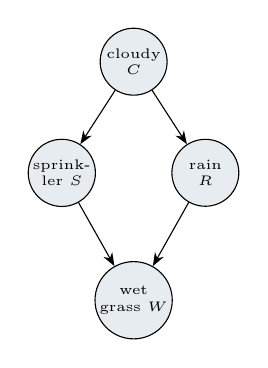
\begin{tikzpicture}[>=Stealth, font=\tiny, node distance=7mm,
	   v/.style={draw, circle, fill=blau-upc!12, inner sep=0.5pt, minimum size=8.5mm, align=center}]
	  \node[v] (C) {cloudy\\ $C$};
	  \node[v, below left=8mm and 3mm of C] (S) {sprink-\\ler $S$};
	  \node[v, below right=8mm and 3mm of C] (R) {rain\\ $R$};
	  \node[v, below=21mm of C] (W) {wet\\ grass $W$};
	  \draw[->] (C)--(S); \draw[->] (C)--(R);
	  \draw[->] (S)--(W); \draw[->] (R)--(W);
	\end{tikzpicture}\\[1.5mm]
	{\tiny\itshape cloud cover is a common cause of sprinkler use and rain}
	\end{center}
	\end{column}
	\end{columns}
}

\frame{\frametitle{Causal decision theory: seeing vs.\ doing}
	\begin{columns}[T]
	\begin{column}{0.60\textwidth}
	\begin{block}{The $\mathrm{do}$-operator}
		{\tiny
		\begin{itemize}
			\item Pearl's key distinction: \emph{observing} $X{=}x$ (passive evidence, as in EDT) is not the same as \emph{doing} $X{=}x$ (an intervention).
			\item $\mathrm{do}(X=x)$: \textbf{sever all arrows into $X$} (cut $X$ off from its causes), fix $X=x$, propagate downstream. Adjusting over the direct causes $z=\mathrm{Pa}(X)$:
			$$P\big(Y \mid \mathrm{do}(X{=}x)\big) = \sum_{z} P(Y\mid x, z)\,P(z).$$
			\item Sprinkler graph: \emph{seeing} the sprinkler on raises the chance it was cloudy, hence lowers the chance of rain. \emph{Doing} $\mathrm{do}(S{=}\text{on})$ cuts $C\to S$, so it tells you \textbf{nothing} about rain.
			\item \textbf{CDT:} $a^{*} = \arg\max_a \mathbb{E}[U \mid \mathrm{do}(A=a)]$ -- judge each action by the causal consequences of \emph{intervening} on it, holding the rest of the past fixed.
			\item The contrast in one line: $\;\mathbb{E}[U\mid \mathrm{do}(A{=}a)]$ (CDT, severs the action's causes) vs.\ $\;\mathbb{E}[U\mid A{=}a]$ (EDT, keeps them as evidence).
		\end{itemize}
		}
	\end{block}
	\end{column}
	\begin{column}{0.40\textwidth}
	\begin{center}
	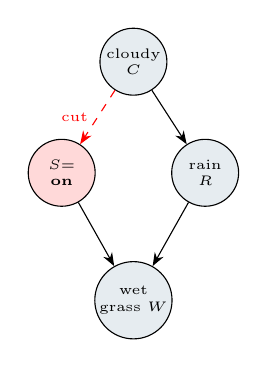
\begin{tikzpicture}[>=Stealth, font=\tiny, node distance=7mm,
	   v/.style={draw, circle, fill=blau-upc!12, inner sep=0.5pt, minimum size=8.5mm, align=center}]
	  \node[v] (C) {cloudy\\ $C$};
	  \node[v, fill=red!15, below left=8mm and 3mm of C] (S) {$S{=}$\\ \textbf{on}};
	  \node[v, below right=8mm and 3mm of C] (R) {rain\\ $R$};
	  \node[v, below=21mm of C] (W) {wet\\ grass $W$};
	  \draw[->, red, dashed] (C)--(S) node[midway, left, font=\tiny, text=red]{cut};
	  \draw[->] (C)--(R);
	  \draw[->] (S)--(W); \draw[->] (R)--(W);
	\end{tikzpicture}\\[1.5mm]
	{\tiny\itshape $\mathrm{do}(S{=}\text{on})$ severs $S$ from its cause $C$}
	\end{center}
	\end{column}
	\end{columns}
}

%==================================================================
\section{CDT and EDT as sequential prediction}
%==================================================================

\frame{\frametitle{Prerequisites: the sequential prediction setting}
	\begin{block}{Histories, environments as chronological semimeasures, and beliefs}
		{\tiny
		\begin{itemize}
			\item Interaction: at each step $t$ the agent emits an action $a_t\in\mathcal{A}$ and receives a percept $e_t\in\mathcal{E}$ (e.g.\ $e_t=(o_t,r_t)$). The history is $h_{<t}=a_1 e_1\cdots a_{t-1}e_{t-1}$.
			\item An \textbf{environment} is a \textbf{chronological semimeasure} $\rho$: it gives the probability of percepts \emph{given} actions,
			$$\rho(e_{1:t}\,\|\,a_{1:t})\in[0,1],$$
			where the double bar $\|$ marks the actions as \textbf{conditioned-on inputs, never predicted}.
			\begin{itemize}\scriptsize
				\item[--] \emph{chronological:} $e_{1:t}$ may depend on $a_{1:t}$ but not on \emph{future} actions;
				\item[--] \emph{semimeasure:} $\sum_{e_t}\rho(e_{1:t}\|a_{1:t})\le\rho(e_{<t}\|a_{<t})$ (probability may leak; a measure has equality).
			\end{itemize}
			\item The agent's belief is a \textbf{Bayesian mixture} over a class $\mathcal{M}$ of environments, $\;\xi(e_{<t}\|a_{<t})=\sum_{\nu\in\mathcal{M}}w_\nu\,\nu(e_{<t}\|a_{<t})$ (AIXI: $\mathcal{M}=$ lower-semicomputable $\nu$, $w_\nu=2^{-K(\nu)}$).
			\item Decision-theoretic crux: \textbf{when the agent chooses $a_t$, does that choice update its belief about which environment it is in?} The answer separates CDT from EDT.
		\end{itemize}
		}
	\end{block}
}

\frame{\frametitle{Chronological semimeasure $=$ CDT}
	\begin{block}{The action is an intervention, not evidence}
		{\tiny
		\begin{itemize}
			\item In a chronological semimeasure the action appears \textbf{only to the right of $\|$}: $\rho$ assigns \emph{no} probability to actions, so ``the action as evidence about $\rho$'' is not even definable.
			\item The posterior over environments updates on \textbf{percepts only}, holding the actions fixed as given:
			$$w_\nu(h_{<t}) \;=\; w_\nu\,\frac{\nu(e_{<t}\,\|\,a_{<t})}{\xi(e_{<t}\,\|\,a_{<t})}.$$
			Choosing $a_t$ does \textbf{not} reweight $w_\nu$: \emph{you do not update ``which environment am I in'' by deciding.}
			\item So the agent evaluates an action by \emph{intervening} and propagating through a \emph{fixed} which-world belief:
			$$a_t \;=\; \arg\max_{a}\ \sum_{e_t}\xi(e_t\,\|\,h_{<t}\,a)\,\big[r_t+\cdots\big] \;=\; \arg\max_a \mathbb{E}_\xi\big[\,U \,\|\, \mathrm{do}(a)\,\big].$$
			\item This is exactly \textbf{CDT}: the chronological bar $\|$ \emph{is} the do-operator, lifted to whole histories. (Newcomb: such an agent two-boxes -- the prediction is a fixed past percept, untouched by $\mathrm{do}(a)$.)
		\end{itemize}
		}
	\end{block}
}

\frame{\frametitle{Joint prediction $=$ EDT}
	\begin{block}{Actions predicted exactly like observations}
		{\tiny
		\begin{itemize}
			\item Now model the \emph{entire} history $h=a_1 e_1 a_2 e_2\cdots$ as \textbf{one stream to predict} over $(\mathcal{A}\times\mathcal{E})^{*}$ -- actions get probabilities too. Take the generative model to be a mixture over (world $\nu$, policy $\pi$) pairs:
			$$P(h_{1:t}) \;=\; \sum_{\nu,\pi} w_{\nu,\pi}\prod_{k=1}^{t}\pi(a_k\mid h_{<k})\,\nu(e_k\mid h_{<k}a_k).$$
			(Solomonoff's $M(h)=\sum_{p:U(p)=h*}2^{-\ell(p)}$ is the universal such joint predictor.)
			\item Choosing/observing $a_t$ is now ordinary \textbf{evidence}: Bayes updates the joint posterior over \emph{both} the policy and the world,
			$$w_{\nu,\pi}(h_{<t}\,a_t)\ \propto\ w_{\nu,\pi}\,\Big[\textstyle\prod_{k<t}\cdots\Big]\,\pi(a_t\mid h_{<t}).$$
			The factor $\pi(a_t\mid h_{<t})$ tells you ``\textbf{what policy am I running}''; and any world $\nu$ \emph{correlated with the action in the prior} $w_{\nu,\pi}$ is reweighted -- ``\textbf{what world am I in}''.
			\item So the agent evaluates an action by \emph{conditioning}: $\;a_t = \arg\max_a \mathbb{E}_P[\,U \mid A_t{=}a,\ h_{<t}\,]$.
			\item This is exactly \textbf{EDT} -- and it reproduces the smoking lesion: the prior correlates the lesion (a world-feature) with the smoking disposition (a policy-feature), so conditioning on ``I smoke'' upweights lesion-worlds and the act looks like bad news, though it is no lever.
		\end{itemize}
		}
	\end{block}
}

%==================================================================
\section{Where CDT and EDT fail}
%==================================================================

\frame{\frametitle{Newcomb's problem: CDT two-boxes, EDT one-boxes}
	\begin{columns}[T]
	\begin{column}{0.60\textwidth}
	\begin{block}{The same problem splits the two rules}
		{\tiny
		\begin{itemize}
			\item \textbf{Newcomb:} a transparent box holds \$1{,}000; an opaque box holds \$1{,}000{,}000 \emph{iff} a highly reliable predictor $\Omega$ foresaw you would take \emph{only} the opaque box. $\Omega$ has already chosen.
			\item \textbf{CDT} applies $\mathrm{do}(A)$: this \textbf{severs} your action from your disposition $S$, so it no longer informs $\Omega$'s prediction $P$. The contents are fixed; taking both boxes earns \$1{,}000 more \emph{in every fixed state}. CDT \textbf{two-boxes} and predictably walks away with \$1{,}000.
			\item \textbf{EDT} conditions: one-boxing is strong \emph{evidence} the opaque box is full, so $\mathbb{E}[U\mid\text{one-box}]$ is huge. EDT \textbf{one-boxes} and gets \$1{,}000{,}000 -- it keeps exactly the predictive dependence CDT discards.
			\item \textbf{Verdict:} CDT loses Newcomb. (In the lens above: the chronological-semimeasure agent two-boxes; the joint-prediction agent one-boxes.)
		\end{itemize}
		}
	\end{block}
	\end{column}
	\begin{column}{0.40\textwidth}
	\begin{center}
	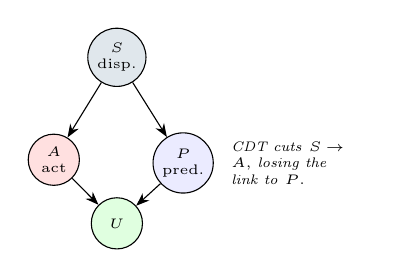
\begin{tikzpicture}[>=Stealth, font=\tiny, node distance=6mm,
	   v/.style={draw, circle, inner sep=1.2pt, minimum size=6.5mm, align=center}]
	  \node[v, fill=blau-upc!15] (S) {$S$\\ disp.};
	  \node[v, fill=red!12, below left=8mm and 3mm of S] (A) {$A$\\ act};
	  \node[v, fill=blue!8, below right=8mm and 3mm of S] (P) {$P$\\ pred.};
	  \node[v, fill=green!12, below=14mm of S] (U) {$U$};
	  \draw[->] (S)--(A); \draw[->] (S)--(P);
	  \draw[->] (A)--(U); \draw[->] (P)--(U);
	  \node[font=\tiny, right=1mm of P, text width=1.6cm] {\textit{CDT cuts} $S\!\to\!A$, \textit{losing the link to} $P$.};
	\end{tikzpicture}
	\end{center}
	\end{column}
	\end{columns}
}

\frame{\frametitle{EDT mistakes evidence for control}
	\begin{block}{The smoking lesion}
		{\tiny
		\begin{itemize}
			\item A genetic lesion $L$ causes cancer (cost $C$) \emph{and} makes you more likely to want to smoke. Smoking itself is harmless and gives benefit $b>0$.
			\item Conditioning on ``I smoke'' raises $P(L)$, hence raises estimated cancer risk: $\mathbb{E}[U\mid \text{smoke}] = b - C\,P(L\mid\text{smoke})$. For strong correlation, EDT \textbf{abstains} -- even though abstaining does \emph{nothing} to reduce cancer. EDT confuses a \textbf{symptom} for a \textbf{lever}.
			\item \textbf{Scorecard:} CDT and EDT are each half right.
			\begin{itemize}\scriptsize
				\item[--] CDT ignores predictive dependence $\Rightarrow$ loses Newcomb.
				\item[--] EDT overreacts to mere correlation $\Rightarrow$ loses the smoking lesion.
			\end{itemize}
			\item The missing ingredient is a dependence that is neither raw physical causation nor raw evidential correlation.
		\end{itemize}
		}
	\end{block}
}

\frame{\frametitle{CDT vs.\ physics: the intervention is a fiction}
	\begin{block}{Does CDT really ``reflect physical reality''? (following Ebtekar \& Hutter)}
		{\tiny
		\begin{itemize}
			\item CDT's $\mathrm{do}(A=a)$ holds the past fixed, \textbf{magically sets the action}, and propagates forward. What licenses cutting the action loose from its causes?
			\item In a \emph{deterministic, time-reversible} physical world, your action has physical antecedents (your brain state, your source code). A predictor that reads those antecedents is correlated with your action through \textbf{perfectly ordinary physics}, not magic.
			\item ``Severing the incoming arrows to $A$'' directly \textbf{contradicts embeddedness}: it pretends your action has no causes, but physically it does. The intervention is a harmless idealisation for a dualistic agent; for an embedded agent it \emph{throws away real correlations} (with predictors, copies, simulations).
			\item So the usual defence is backwards: physics gives no privileged metaphysical ``intervention'' that frees the action from its past. This pressures us to move the counterfactual off the \emph{physical act} and onto the agent's \emph{policy / computation}.
		\end{itemize}
		}
	\end{block}
}

\frame{\frametitle{Spurious counterfactuals: EDT breaks for self-aware agents}
	\begin{block}{Conditioning on a probability-zero action}
		{\tiny
		\begin{itemize}
			\item A capable embedded agent can reason about (even \emph{prove} things about) its own source code, so it can largely predict its own action. But then, for the action $a$ it will \emph{not} take, $P(A=a)=0$.
			\item EDT's recipe $\mathbb{E}[U\mid A=a]$ is then $\tfrac{0}{0}$ -- \textbf{undefined}. You may assign the unchosen action \emph{any} value you like: a \textbf{spurious counterfactual}.
			\item So conditioning gives \emph{no constraint} on counterfactual actions you are certain you won't take -- exactly the cases decision-making turns on.
			\item (Foreshadow: in proof-theoretic form this same pathology becomes the \textbf{5-and-10 problem}, and the fix needs a notion of \emph{logical} dependence.)
		\end{itemize}
		}
	\end{block}
}

%==================================================================
\section{Functional \& updateless decision theory}
%==================================================================

\frame{\frametitle{Functional decision theory: choose your function's output}
	\begin{block}{``Which output of this very function would yield the best outcome?''}
		{\tiny
		\begin{itemize}
			\item Reframe \emph{what you are choosing}. You are not just \emph{this body about to act}; you are running a fixed \textbf{decision function}, and your action is its \emph{output} on the situation you face.
			\item Many things in the world may depend on that \emph{same} function: a predictor who \textbf{modelled} it, a \textbf{copy} of you running it, a simulation of it. When the function's output changes, all of them change \emph{with} it.
			\item So FDT does not ask ``what should I do, holding everything else fixed?'' (that is CDT). It asks the question the paper puts at its centre:
			\begin{center}\emph{``which output of this very decision function -- given everything in the world that depends on it -- would yield the best outcome?''}\end{center}
			and then \emph{returns that output}. Concretely: score each candidate action $a$ by the outcome in the world where \emph{my decision function outputs $a$} (so the predictor predicted $a$, and every copy outputs $a$), and take the best.
			\item It acts \emph{as if it controls all instances of the computation at once} -- not by magic, but because they really are the same logical fact.
			\item This wins the earlier cases for the \emph{right} reason: in Newcomb the prediction tracks the function's output, so FDT \textbf{one-boxes}; the lesion does \emph{not} run the function, so FDT still \textbf{smokes}. FDT shines exactly where embedded agents live -- worlds containing copies of you, or predictors that model your decision procedure.
		\end{itemize}
		}
	\end{block}
}

\frame{\frametitle{Twin Prisoner's Dilemma \& subjunctive dependence}
	\begin{columns}[T]
	\begin{column}{0.58\textwidth}
	\begin{block}{Same function, two bodies}
		{\tiny
		\begin{itemize}
			\item You and a psychological \emph{twin} (your exact copy) play a one-shot Prisoner's Dilemma in separate rooms, no communication. You run the \emph{same} decision function.
			\item \textbf{CDT:} ``I can't causally affect her; defection dominates.'' Both defect, each gets \$1.
			\item \textbf{FDT:} ``We compute the same function. If it outputs $C$, both cooperate; if $D$, both defect.'' So FDT cooperates -- both get \$3.
			\item \textbf{Subjunctive dependence} (Y\&S): when two physical systems compute the \emph{same} function, their outputs are logically tied -- like two calculators evaluating $6288{+}1048$: see one print $7336$ and you know the other will too. Causal dependence is a \emph{special case}; mere correlation (both calculators happen to be pink) is not. FDT acts as if it controls \emph{all} instances of the computation at once.
		\end{itemize}
		}
	\end{block}
	\end{column}
	\begin{column}{0.42\textwidth}
	\begin{center}
	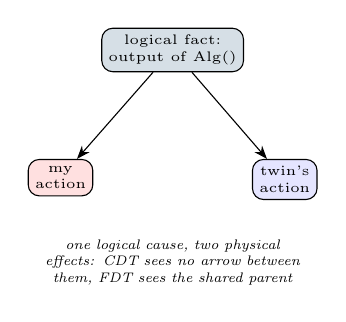
\begin{tikzpicture}[>=Stealth, font=\tiny, node distance=7mm,
	   b/.style={draw, rounded corners, inner sep=2.5pt, align=center}]
	  \node[b, fill=blau-upc!20] (alg) {logical fact:\\ output of $\mathrm{Alg}()$};
	  \node[b, fill=red!12, below left=11mm and 1mm of alg] (me) {my\\ action};
	  \node[b, fill=blue!10, below right=11mm and 1mm of alg] (tw) {twin's\\ action};
	  \draw[->] (alg)--(me); \draw[->] (alg)--(tw);
	  \node[font=\tiny\itshape, below=20mm of alg, text width=3.4cm, align=center]
	    {one logical cause, two physical effects: CDT sees no arrow between them, FDT sees the shared parent};
	\end{tikzpicture}
	\end{center}
	\end{column}
	\end{columns}
}

\frame{\frametitle{Counterfactual mugging: the updateless move}
	\begin{columns}[T]
	\begin{column}{0.58\textwidth}
	\begin{block}{Paying in a branch you know you're not rewarded in}
		{\tiny
		\begin{itemize}
			\item $\Omega$ flips a fair coin. \textbf{Tails:} you get $R=\$10{,}000$ iff $\Omega$ predicted you'd pay on heads. \textbf{Heads:} $\Omega$ asks for $c=\$100$. You are asked to pay (so: heads). Pay?
			\item \textbf{Updateful} reasoning conditions on ``I'm in heads'': it sees only the \$100 cost and \textbf{refuses}. But \emph{ex ante} the policy ``pay if asked'' is worth $\tfrac12(R-c)>0$.
			\item \textbf{UDT 1.0:} evaluate the local output against the \textbf{prior} -- keep the (tails) branch whose payoff your policy controls, by dropping the updateful rule's extra $O{=}o$ conditioning:
			$$\mathrm{choice}(o)=\arg\max_a \mathbb{E}\big[U\mid \mathrm{choice}(o){=}a\big].$$
			So UDT 1.0 \textbf{pays}.
			\item Updatelessness is \emph{not} ignorance (no predictor $\Rightarrow$ UDT $=$ ordinary EU max), and it is \emph{reflectively stable}: the agent already follows the policy it would have precommitted to.
		\end{itemize}
		}
	\end{block}
	\end{column}
	\begin{column}{0.42\textwidth}
	\begin{center}
	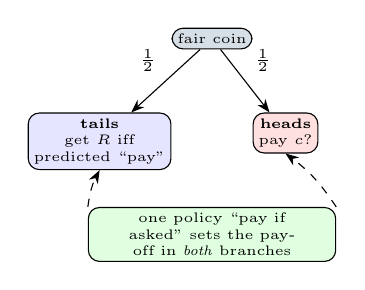
\begin{tikzpicture}[>=Stealth, font=\tiny, node distance=6mm,
	   b/.style={draw, rounded corners, inner sep=2pt, align=center}]
	  \node[b, fill=blau-upc!20] (c) {fair coin};
	  \node[b, fill=blue!10, below left=8mm and 0mm of c] (T) {\textbf{tails}\\ get $R$ iff\\ predicted ``pay''};
	  \node[b, fill=red!12, below right=8mm and 0mm of c] (H) {\textbf{heads}\\ pay $c$?};
	  \draw[->] (c)--(T) node[midway,above left,font=\tiny] {$\tfrac12$};
	  \draw[->] (c)--(H) node[midway,above right,font=\tiny] {$\tfrac12$};
	  \node[b, fill=green!12, below=20mm of c, text width=3cm, align=center] (pol)
	    {one policy ``pay if asked'' sets the payoff in \emph{both} branches};
	  \draw[->, dashed] (pol.north west) to[bend left=10] (T.south);
	  \draw[->, dashed] (pol.north east) to[bend right=10] (H.south);
	\end{tikzpicture}
	\end{center}
	\end{column}
	\end{columns}
}

\frame{\frametitle{UDT 1.1: optimise the whole policy, not one action}
	\begin{columns}[T]
	\begin{column}{0.57\textwidth}
	\begin{block}{When local outputs must be coordinated}
		{\tiny
		\begin{itemize}
			\item Even \emph{updateless local-action} selection can be too local. \textbf{Copied-agent anti-coordination}: two copies see index $1$ or $2$, must pick \emph{different} actions to win (10 each), else 0.
			\item The local question ``if $\mathrm{Alg}(1)=A$, what is $\mathrm{Alg}(2)$?'' is the \emph{wrong type}: both symmetric answers fail. The good object is the \emph{whole table} $\mathrm{Alg}:\{1,2\}\to\{A,B\}$.
			\item \textbf{UDT 1.1 (Wei Dai):} first choose the entire \emph{policy} (a map $S:O\to A$) against the prior, \emph{then} apply $S^{*}$ to your actual observation $o$:
			$$S^{*}\in\arg\max_{S:\,O\to A}\ \mathbb{E}\big[U\mid \mathrm{choice}{=}S\big].$$
			(UDT 1.0 instead fixes a single \emph{output} and hopes the rest fall out right.)
			\item $\pi_{AB},\pi_{BA}$ score 10; a shared tie-breaker coordinates the copies. This is \textbf{global optimisation over branches}, not local optimisation.
		\end{itemize}
		}
	\end{block}
	\end{column}
	\begin{column}{0.43\textwidth}
	\begin{center}
	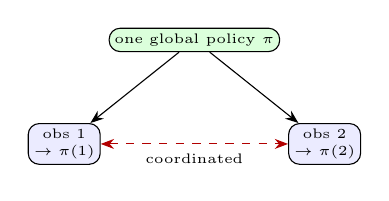
\begin{tikzpicture}[>=Stealth, font=\tiny,
	   b/.style={draw, rounded corners, inner sep=2pt, align=center}]
	  \node[b, fill=green!14] (pi) {one global policy $\pi$};
	  \node[b, fill=blue!8, below left=9mm and 1mm of pi] (o1) {obs $1$\\ $\to\pi(1)$};
	  \node[b, fill=blue!8, below right=9mm and 1mm of pi] (o2) {obs $2$\\ $\to\pi(2)$};
	  \draw[->] (pi)--(o1); \draw[->] (pi)--(o2);
	  \draw[<->, dashed, red!70!black] (o1)--(o2) node[midway,below,font=\tiny,text=black]{coordinated};
	\end{tikzpicture}
	\end{center}
	\end{column}
	\end{columns}
}

\frame{\frametitle{The three shifts in ``what am I choosing?''}
	\begin{block}{CDT/EDT $\to$ FDT $\to$ UDT 1.0 $\to$ UDT 1.1 (after Kosoy's formalism)}
		{\tiny
		\begin{center}
		\renewcommand{\arraystretch}{1.3}
		\begin{tabular}{l|l|l|l}
		\textbf{Rule} & \textbf{Object chosen} & \textbf{Update status} & \textbf{Dependence used}\\
		\hline
		CDT & local physical act & updateful & causal intervention\\
		EDT & local act (as evidence) & updateful & evidential correlation\\
		FDT / TDT & local algorithm output & updateful & logical / subjunctive\\
		UDT 1.0 & local algorithm output & \textbf{updateless} & logical / subjunctive\\
		UDT 1.1 & \textbf{whole policy} & updateless & logical over policies\\
		\end{tabular}
		\end{center}
		\begin{itemize}
			\item \textbf{Shift 1 (FDT):} from a physical act to the output of an abstract computation -- captures predictors, copies, simulations.
			\item \textbf{Shift 2 (UDT 1.0):} from posterior to prior -- keep the value of being predictable, don't discard branches whose payoff your policy controls.
			\item \textbf{Shift 3 (UDT 1.1):} from a single output to a whole policy -- coordinate behaviour across all possible observations.
		\end{itemize}
		}
	\end{block}
}

%==================================================================
\section{Problems with UDT}
%==================================================================

\frame{\frametitle{Problem 1: paying for worlds that don't exist}
	\begin{block}{Ex-ante optimality is only as good as the prior}
		{\tiny
		\begin{itemize}
			\item UDT maximises \emph{prior} expected utility. In the branch it actually inhabits it will \textbf{knowingly burn real utility}. In counterfactual mugging, after seeing heads, UDT hands over a real \$100 in the only world it will ever experience, to benefit a tails-world \emph{it now knows did not happen}.
			\item Generalise: a UDT agent will take actions that are bad \emph{in the actual world} because they would have been good in counterfactual scenarios that are never realised.
			\item This is dangerous when the prior is even slightly wrong about \emph{which worlds are possible}: put prior mass on a predictor that does not actually exist (or on a logically impossible scenario), and UDT pays a \textbf{real, ongoing tax} for fake benefits. A clever (or merely hypothetical) $\Omega$ can extract resources by promising/threatening in branches that never occur.
			\item The worry: is ``best from the prior'' the right notion of rational, when ``the prior'' ranges over worlds you have since learned are not actual?
		\end{itemize}
		}
	\end{block}
}

\frame{\frametitle{Problem 2: logical updatelessness}
	\begin{block}{Which prior, when some of your uncertainty is mathematical?}
		{\tiny
		\begin{itemize}
			\item A real embedded agent's uncertainty is not only \emph{empirical} (coin flips). It is also \textbf{logical}: it does not know all consequences of its own source code, the $10^{100}$-th digit of $\pi$, or whether the opponent's program halts.
			\item UDT says ``don't update.'' Refusing to update on \emph{empirical} observations is clear. Refusing to update on \emph{logical} facts is not: as the agent thinks longer it \emph{learns} logical facts (proves theorems, computes digits) -- and that looks exactly like updating.
			\item \textbf{Logical updatelessness} would have the agent choose its policy as if from a state of \emph{logical} ignorance, not taking computed logical facts into account. But (a) it cannot help computing some of them, and (b) we have \textbf{no coherent ``logical prior''} -- a probability distribution over mathematical truths before any computation.
			\item This is open. A satisfactory UDT needs a theory of \emph{logical uncertainty} (cf.\ logical induction), which we do not yet have. It is also the doorway to the 5-and-10 problem.
		\end{itemize}
		}
	\end{block}
}

%==================================================================
\section{The 5-and-10 problem}
%==================================================================

\frame{\frametitle{The 5-and-10 problem}
	\begin{columns}[T]
	\begin{column}{0.45\textwidth}
	\begin{block}{Two programs (Demski \& Garrabrant)}
		{\tiny
		Take \$5 or \$10; utility is the dollars taken, so take \$10. The agent has its own source code and the world's, and chooses by proof search.\\[1.5mm]
		{\ttfamily\scriptsize
		\begin{tabular}{@{}l@{}}
		U():\\
		~~if A() = 10: return 10\\
		~~if A() = 5:~~return 5\\[1.6mm]
		A():\\
		~~search for a proof of\\
		~~~~[A()=5 -> U()=x] and\\
		~~~~[A()=10 -> U()=y],\\
		~~~~for x,y in \{0,5,10\}\\
		~~if found, x>y: return 5\\
		~~else: return 10\\
		\end{tabular}}
		}
	\end{block}
	\end{column}
	\begin{column}{0.55\textwidth}
	\begin{block}{Why it returns \$5}
		{\tiny
		\begin{itemize}
			\item The world returns whatever the agent returns, so \$10 genuinely beats \$5. Yet with enough search time \texttt{A} returns \$5.
			\item Let $P$ be the sentence ``$[\texttt{A()=5}\Rightarrow\texttt{U()=5}]$ and $[\texttt{A()=10}\Rightarrow\texttt{U()=0}]$''.
			\item \textbf{A proof of $P$ makes $P$ true.} If $P$ is proved, \texttt{A} finds it ($x{=}5>y{=}0$) and returns \$5. Then \texttt{A()=5}, so the first conjunct holds; and \texttt{A()=10} is false, so the second holds \emph{vacuously} (a false ``if'' implies anything). Hence $P$.
			\item So $\Box P\to P$ is itself provable ($\Box X$ means ``$X$ is provable''). \textbf{L\"ob's theorem} ($\Box(\Box P\to P)\to\Box P$) then makes $P$ provable; the search finds it and returns \$5.
			\item \textbf{Spurious proof:} \texttt{A} takes \$5 because it proves that taking \$10 pays \$0, and that holds \emph{only because} it takes \$5. The action not taken is provably false, and an ``if'' with a false premise carries no information, so ordinary counterfactuals over one's own action break down.
		\end{itemize}
		}
	\end{block}
	\end{column}
	\end{columns}
}


%==================================================================
\section{A formal criterion for decision theories}
%==================================================================

\frame{\frametitle{Why we want a formal optimality criterion}
	\begin{block}{Beyond case-by-case scoring}
		{\tiny
		\begin{itemize}
			\item Newcomb, counterfactual mugging, the 5-and-10 problem, the twin PD, open-source games all share a \textbf{common structure}: agent and environment are both \emph{programs} that may inspect each other's code, simulate each other's behaviour, or contain subroutines algorithmically \emph{isomorphic} to one another.
			\item Yet these are usually presented as standalone puzzles, and CDT/EDT/FDT/UDT are judged \emph{case by case} (``does it get Newcomb right?'') rather than against a single optimality standard.
			\item \textbf{The substantive question:} can we define one class of computational environments rich enough to contain all these problems at once, together with a criterion of optimality that any candidate decision theory can be \emph{measured} against?
		\end{itemize}
		}
	\end{block}
}

\frame{\frametitle{Agents and worlds as programs}
	\begin{columns}[T]
	\begin{column}{0.56\textwidth}
	\begin{block}{The setup}
		{\tiny
		\begin{itemize}
			\item \textbf{Agent} $=$ a program with access to (i) its own source code and (ii) the world's source code; it returns an action.
			\item \textbf{World} $=$ a program that may
			\begin{itemize}\scriptsize
				\item[--] \emph{call the agent} as a function (input $\to$ action), possibly \emph{many times on different inputs} (``what would the agent do if it observed $x$?''), and
				\item[--] \emph{search for proofs} about the agent's input--output behaviour;
			\end{itemize}
			it returns a utility.
			\item \textbf{Goal:} design an agent whose utility is high across (almost) all worlds -- the best mapping from situations to actions.
		\end{itemize}
		}
	\end{block}
	\end{column}
	\begin{column}{0.44\textwidth}
	\begin{center}
	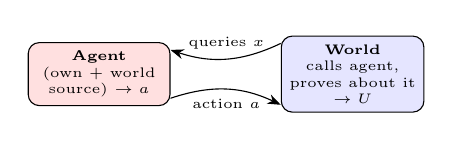
\begin{tikzpicture}[>=Stealth, font=\tiny,
	   b/.style={draw, rounded corners, align=center, inner sep=3pt, minimum height=8mm}]
	  \node[b, fill=red!12, minimum width=18mm] (ag) {\textbf{Agent}\\ (own + world\\ source) $\to a$};
	  \node[b, fill=blue!10, minimum width=18mm, right=14mm of ag] (wo) {\textbf{World}\\ calls agent,\\ proves about it\\ $\to U$};
	  \draw[->] ($(wo.north west)+(0,-1mm)$) to[bend left=22] node[above,font=\tiny]{queries $x$} ($(ag.north east)+(0,-1mm)$);
	  \draw[->] ($(ag.south east)+(0,1mm)$) to[bend left=22] node[below,font=\tiny]{action $a$} ($(wo.south west)+(0,1mm)$);
	\end{tikzpicture}
	\end{center}
	\end{column}
	\end{columns}
}

\frame{\frametitle{Fairness}
	\begin{block}{Judging the agent only on its behaviour}
		{\tiny
		\begin{itemize}
			\item Without a constraint, a ``world'' could just punish source code: ``if the agent is written in Python, utility $=0$.'' Then \emph{no} decision theory could do well and the criterion would be vacuous.
			\item \textbf{Fairness:} the world may depend on the agent \emph{only through its input--output behaviour} (its policy), never through implementation details unrelated to its outputs. Equivalently, a fair world is representable as a program that takes the agent's \emph{policy/behaviour} as input.
			\item Newcomb, the smoking lesion, counterfactual mugging, the twin PD, and the open-source PD are all \textbf{fair}: the predictor/lesion/copy interacts with the agent through its behaviour. This is what makes them legitimate tests.
		\end{itemize}
		}
	\end{block}
}

\frame{\frametitle{What a good agent must discover}
	\begin{block}{Two demands -- which are exactly FDT/UDT turned into a spec}
		{\tiny
		\begin{itemize}
			\item \textbf{Coordinate across function calls.} If the world queries the agent on several inputs (probing its counterfactual behaviour), the agent must \emph{recognise this} and keep its counterfactual outputs \emph{coordinated} for high utility. (This is precisely UDT 1.1's move to optimise a whole policy.)
			\item \textbf{Subjunctive dependence.} If the world contains a subroutine \emph{algorithmically isomorphic} to the agent (a copy in different code), the agent should treat its own decision as also fixing that subroutine's output -- and so must \emph{detect} that ``the world contains something isomorphic to me.'' (This is precisely FDT.)
		\end{itemize}
		}
	\end{block}
	\begin{block}{The open problem (and the bridge ahead)}
		{\tiny
		\begin{itemize}
			\item Define the class of fair computational worlds precisely; define optimality (e.g.\ dominance across all fair worlds); show CDT/EDT/FDT/UDT differ on it; and ask whether any (or some modification) is \emph{optimal}.
			\item Caveats already met: logical counterfactuals (5-and-10), logical uncertainty / logical updatelessness, what counts as a ``policy'', and multi-agent fairness \& bargaining -- which lead into reflective oracles, open-source games, and commitment races.
		\end{itemize}
		}
	\end{block}
}

\end{document}
